\begin{appendices}

\chapter{Transactions and Blocks}
Querying a node for transactions:
\begin{figure}[H]
    \centering
    \lstinputlisting{code/transaction_example.json}
    \caption{Contents of an Ethereum transaction when querying a node}
    \label{fig:transaction}
\end{figure}

Querying a node for block contents:
\begin{figure}[H]
    \centering
    \lstinputlisting{code/block_example.json}
    \caption{Contents of an Ethereum block when querying a node}
    \label{fig:block}
\end{figure}

Ganache UI:
\begin{figure}[H]
    \centering
    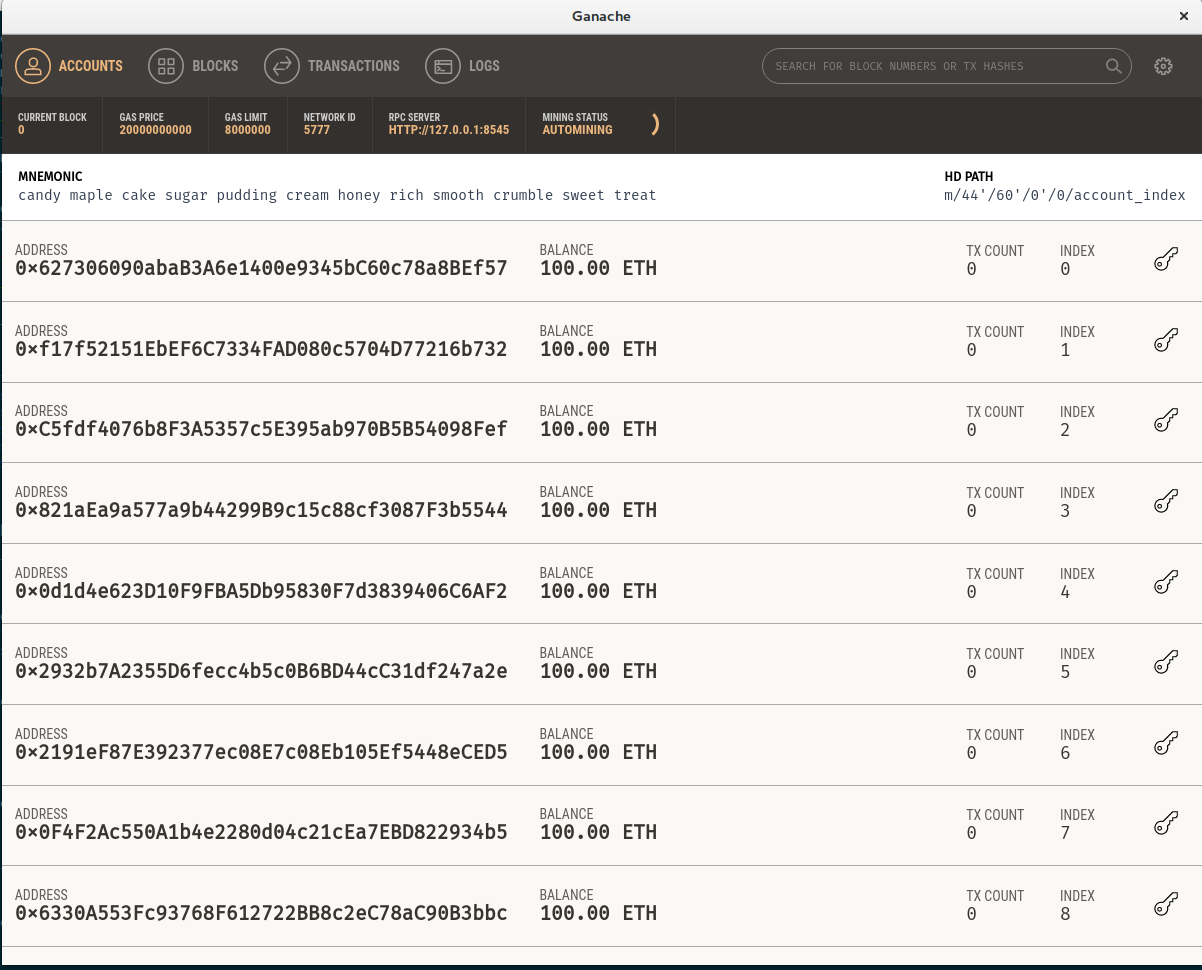
\includegraphics[width=1.0\textwidth]{ganache}
    \caption{Ganache testnet User Interface}
    \label{fig:ganache}
    
\end{figure}

Web3js example:
\begin{figure}[H]
    \centering
    \lstinputlisting{code/web3.js}
    \caption{Interacting with a node in Javascript}
    \label{fig:web3js}
\end{figure}

Web3py example:
\begin{figure}[H]
    \centering
    \lstinputlisting{code/web3.py}
    \caption{Interacting with a node in Python}
    \label{fig:web3py}
\end{figure}

\chapter{Scalability through Gas Saving masks} \label{apx:scalability}

\begin{figure}[ht!]
    \centering
    \lstinputlisting[language=Solidity]{contracts/LibraryExample.sol}
    \caption{Example of using the \texttt{using X for Y} syntax to enhance operations done on datatypes.}
    \label{fig:library}
\end{figure}


\begin{figure}[ht!]
    \centering
    \lstinputlisting[language=Solidity]{contracts/LibraryExample.sol}
    \caption{Example of using the \texttt{using X for Y} syntax to enhance operations done on datatypes.}
    \label{apx:scalability:overflow}
\end{figure}

\begin{figure}[H]
  \begin{subfigure}[b]{\textwidth}
    \centering
    \lstinputlisting[language=Solidity]{contracts/Packing.sol}
  \end{subfigure}

  \begin{subfigure}[b]{\textwidth}
    \centering
    \lstinputlisting{code/solc.txt}
  \end{subfigure}
  \caption{Running the optimizer in storage variables less than 256 bytes results in 2 SSTORE commands instead of 6 which reults in significant savings in gas costs}
  \label{fig:struct_optimization}
\end{figure}
Game interface:
\begin{figure}[H]
    \centering
    \lstinputlisting[language=Solidity]{contracts/GameInterface.sol}
    \caption{Interface for described use-case}
    \label{fig:game_interface}
\end{figure}

Tightly packed code:
\begin{figure}[H]
  % Struct Definition
  \begin{subfigure}[b]{\textwidth}
    \centering
    \lstinputlisting[language=Solidity, firstline=4, lastline=13]{contracts/GameTightlyPacked.sol}
    \caption{Character structure definition}
    \label{fig:struct_optimization:a}
  \end{subfigure}

  \begin{subfigure}[b]{\textwidth}
    \centering
    \lstinputlisting[language=Solidity, firstline=38, lastline=66]{contracts/GameTightlyPacked.sol}
    \caption{Create character simply sets values to each struct variable}
    \label{fig:struct_optimization:b}
  \end{subfigure}
\end{figure}

\begin{figure}[H] \ContinuedFloat
  \begin{subfigure}[b]{\textwidth}
    \centering
    \lstinputlisting[language=Solidity, firstline=68, lastline=92]{contracts/GameTightlyPacked.sol}
    \caption{Retrieve the character and save it in memory, then return all values.}
    \label{fig:struct_optimization:c}
  \end{subfigure}
  \caption{Implementation requires a Solidity `struct' to pack all the variables together. CreateCharacter and GetCharacterStats  }
  \label{fig:struct_optimization}
\end{figure}

Method 2 code:

\begin{figure}[H]
    \centering
    \lstinputlisting[language=Solidity, firstline=10, lastline=36]{contracts/GameByteMasking.sol}
    \caption{Create Character by shifting variables}
    \label{fig:uint_encoding_code}
\end{figure}

\begin{figure}[H] 
    \centering
    \lstinputlisting[language=Solidity, firstline=38, lastline=61]{contracts/GameByteMasking.sol}
    \caption{Get the traits of a character by shifting and masking appropriately. Typecasting is the same as applying a mask of $N$ bits.}
    \label{fig:uint_decoding_code}
\end{figure}

Method 3 code:

\begin{figure}[H]
  \begin{subfigure}[b]{\textwidth}
    \centering
    \lstinputlisting[firstline=35, lastline=41, language=Solidity]{contracts/GameByteMaskingLib.sol}
    \caption{Getting and setting a property}
  \end{subfigure}
  \begin{subfigure}[b]{\textwidth}
    \centering
    \lstinputlisting[linerange={21-21,26-26}, language=Solidity]{contracts/GameByteMaskingLib.sol}
    \caption{Mask and shift offsets for CreationTime}
  \end{subfigure}
  \begin{subfigure}[b]{\textwidth}
    \centering
    \lstinputlisting[linerange={44-44,53-53}, language=Solidity]{contracts/GameByteMaskingLib.sol}
    \caption{Getting and Setting creation time API}
  \end{subfigure}
  \caption{Parts of the Library API for Character Creation}
  \label{apx:scalability:lib}
\end{figure}

\begin{figure}[H]
    \begin{subfigure}[b]{0.5\textwidth}
        \centering
        \lstinputlisting[language=Solidity, linerange={101-108}]{contracts/GameByteMaskingLib.sol}
        \caption{Create Character by shifting variables}
        \label{fig:bytes_encoding_code}
    \end{subfigure}
    \begin{subfigure}[b]{0.5\textwidth}
        \centering
        \lstinputlisting[language=Solidity, linerange={129-139}]{contracts/GameByteMaskingLib.sol}
        \caption{get character variables}
        \label{fig:bytes_decoding_code}
    \end{subfigure}
\end{figure}

\chapter{Security}

\subsection{Deleting a struct with mapping} \label{apx:security:mapping}
\begin{figure}[H]
    \centering
    \lstinputlisting[language=Python]{code/getstorageat.py}
    \caption{Inspecting the first storage slot of a contract}
    \label{fig:storage}
\end{figure}

\chapter{Implementation}

\section{Listening for Events} \label{apx:implementation:events}

\section{Access Control}\label{apx:implementation:acl}
Explain modifiers and whitelist. Compare to having ACL contract.

% The above contract was initialized with 1 ether at its balance. An attack can drain the contract by calling the $GetGift$ function with the correct password. Due to the attacker not knowing the password, they proceed to change it, using the $SetPass$ function, which requires at least a 1 ether deposit, which is acceptable since the attacker will get that back. This also requires that the `passHasBeenSet' variable is false, or that the PassHasBeenSet function has not been called yet.

% A naive attacker would inspect the contract's transactions in Etherscan\footnote{https://etherscan.io/address/0xd8993f49f372bb014fb088eabec95cfdc795cbf6} and after notice that no transaction referring to `PassHasBeenSet' has been made, and thus proceed to attack the contract and change the password, only to find that the password did not get changed. A transaction where a contract calls another contract's function is called a `Message Call'. Etherscan shows this kind of calls as `Internal Transactions', only when they include values of more than 0 ether. In this case, `PassHasBeenSet' does not accept Ether and thus cannot be detected in Etherscan. The contract's owner called `PassHasBeenSet' from another contract and as a result the password is not changeable. Detecting that the `passHasBeenSet' variable had been set to true can be done by inspecting the storage of the smart contract, which is always public as shown in \ref{fig:storage}

\end{appendices}